\documentclass[tikz, border=2mm]{standalone} 

\begin{document}
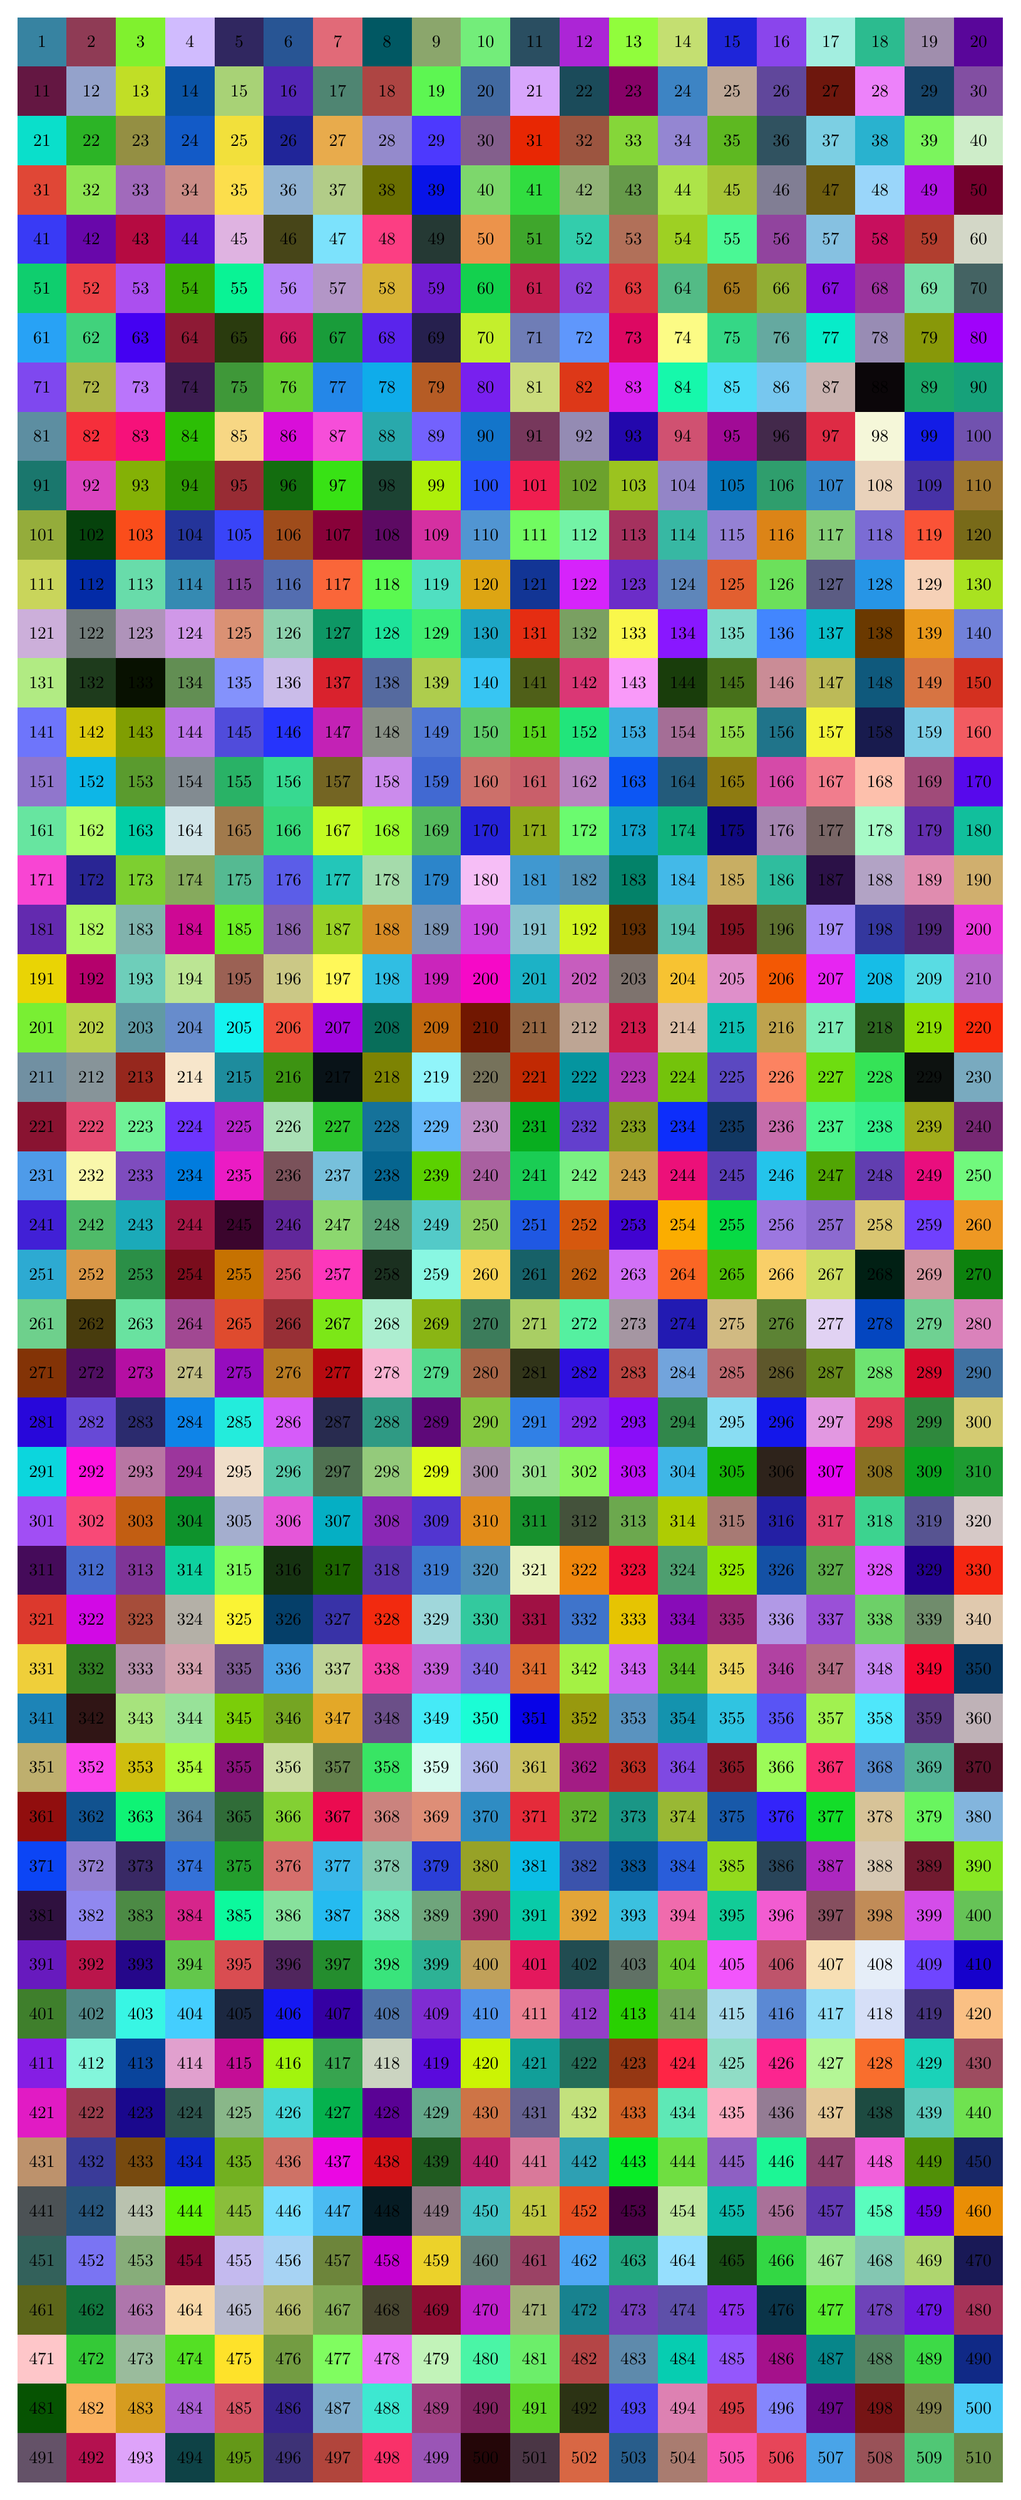
\begin{tikzpicture}[scale=1]
  \foreach \y [count=\ny from 0] in {0.5,1.5,...,49.5} {
      \foreach \x [count=\nx, evaluate=\x as \num using int(\nx+10*\ny)] in {0.5,1.5,...,19.5} {
            \pgfmathsetmacro{\R}{random(0,10000)/10000}%
            \pgfmathsetmacro{\G}{random(0,10000)/10000}%
            \pgfmathsetmacro{\B}{random(0,10000)/10000}%
            \definecolor{MyColor}{rgb}{\R,\G,\B}%
          \node[fill=MyColor,inner sep=0.1cm,outer sep=0pt,anchor=center, minimum size=1cm] at (\x,-\y) {\num}; 
      }
  }
\end{tikzpicture}
\end{document}
